\documentclass{beamer}
\usepackage[utf8]{inputenc}
\usepackage{graphicx, epsfig}
\usepackage{amsmath,mathrsfs,amsfonts,amssymb}
\usepackage{floatflt}
\usepackage{epic,ecltree}
\usepackage{mathtext}
\usepackage{fancybox}
\usepackage{fancyhdr}
\usepackage{multirow}
\usepackage{enumerate}
\usepackage{epstopdf}
\usepackage{multicol}
\usepackage{algorithm}
\usepackage[noend]{algorithmic}
\usepackage{tikz}
\usepackage{blindtext}
\usetheme{default}%{Singapore}%{Warsaw}%{Warsaw}%{Darmstadt}
\usecolortheme{default}

\setbeamerfont{title}{size=\Huge}
\setbeamertemplate{footline}[page number]{}

\setbeamertemplate{section in toc}[sections numbered]


\makeatletter
\newcommand\HUGE{\@setfontsize\Huge{35}{40}}
\makeatother    

\setbeamerfont{title}{size=\HUGE}
\beamertemplatenavigationsymbolsempty

% latin bold lower
\newcommand{\ba}{\mathbf{a}} 
\newcommand{\bc}{\mathbf{c}} 
\newcommand{\be}{\mathbf{e}} 
\newcommand{\bh}{\mathbf{h}} 
\newcommand{\bp}{\mathbf{p}} 
\newcommand{\bt}{\mathbf{t}} 
\newcommand{\bs}{\mathbf{s}} 
\newcommand{\bu}{\mathbf{u}} 
\newcommand{\bv}{\mathbf{v}} 
\newcommand{\bw}{\mathbf{w}} 
\newcommand{\bx}{\mathbf{x}} 
\newcommand{\by}{\mathbf{y}} 
\newcommand{\bz}{\mathbf{z}} 

% latin bold upper
\newcommand{\bA}{\mathbf{A}} 
\newcommand{\bB}{\mathbf{B}} 
\newcommand{\bC}{\mathbf{C}} 
\newcommand{\bI}{\mathbf{I}} 
\newcommand{\bJ}{\mathbf{J}} 
\newcommand{\bL}{\mathbf{L}} 
\newcommand{\bM}{\mathbf{M}} 
\newcommand{\bP}{\mathbf{P}}
\newcommand{\bQ}{\mathbf{Q}} 
\newcommand{\bR}{\mathbf{R}} 
\newcommand{\bT}{\mathbf{T}} 
\newcommand{\bU}{\mathbf{U}} 
\newcommand{\bV}{\mathbf{V}} 
\newcommand{\bW}{\mathbf{W}} 
\newcommand{\bX}{\mathbf{X}} 
\newcommand{\bY}{\mathbf{Y}} 
\newcommand{\bZ}{\mathbf{Z}} 

% latin cal upper
\newcommand{\cF}{\mathcal{F}} 
\newcommand{\cG}{\mathcal{G}} 
\newcommand{\cI}{\mathcal{I}} 
\newcommand{\cL}{\mathcal{L}} 
\newcommand{\cM}{\mathcal{M}} 
\newcommand{\cN}{\mathcal{N}} 
\newcommand{\cP}{\mathcal{P}} 
\newcommand{\cS}{\mathcal{S}} 
\newcommand{\cT}{\mathcal{T}} 
\newcommand{\cW}{\mathcal{W}} 
\newcommand{\cX}{\mathcal{X}} 
\newcommand{\cZ}{\mathcal{Z}} 

% latin bb upper
\newcommand{\bbE}{\mathbb{E}} 
\newcommand{\bbI}{\mathbb{I}} 
\newcommand{\bbP}{\mathbb{P}} 
\newcommand{\bbR}{\mathbb{R}} 

% greek bold lower
\newcommand{\bepsilon}{\boldsymbol{\epsilon}} 
\newcommand{\btheta}{\boldsymbol{\theta}} 
\newcommand{\blambda}{\boldsymbol{\lambda}} 
\newcommand{\bpi}{\boldsymbol{\pi}} 
\newcommand{\bmu}{\boldsymbol{\mu}} 
\newcommand{\bsigma}{\boldsymbol{\sigma}} 
\newcommand{\bphi}{\boldsymbol{\phi}} 

% greek bold upper
\newcommand{\bSigma}{\boldsymbol{\Sigma}} 

\DeclareMathOperator*{\argmin}{arg\,min}
\DeclareMathOperator*{\argmax}{arg\,max}

\newcommand{\createdgmtitle}[1]{\title[\hbox to 56mm{Deep Generative Models  \hfill\insertframenumber\,/\,\inserttotalframenumber}]
	{\vspace{1cm} \\ \textbf{Deep Generative Models} \\ {\Huge Lecture #1}}
	\author{Roman Isachenko}
		\institute{
\includegraphics[width=0.7cm]{../utils/aimasterslogo} \LARGE{AI Masters}}
	\date{2024, Spring}
}

\usepackage{tikz}
\usetikzlibrary{arrows,shapes,positioning,shadows,trees}

\newcommand\myfootnote[1]{%
  \tikz[remember picture,overlay]
  \draw (current page.south west) +(1in + \oddsidemargin,0.5em)
  node[anchor=south west,inner sep=0pt]{\parbox{\textwidth}{%
      \rlap{\rule{10em}{0.4pt}}\raggedright\scriptsize \textit{#1}}};}

\newcommand\myfootnotewithlink[2]{%
  \tikz[remember picture,overlay]
  \draw (current page.south west) +(1in + \oddsidemargin,0.5em)
  node[anchor=south west,inner sep=0pt]{\parbox{\textwidth}{%
      \rlap{\rule{10em}{0.4pt}}\raggedright\scriptsize\href{#1}{\textit{#2}}}};}
      
\AtBeginSection[]
      {
      	\begin{frame}{Outline}
      		\tableofcontents[currentsection]
      	\end{frame}
      }
      \AtBeginSubsection[]{
      	\begin{frame}{Outline}
      		\tableofcontents[currentsection,currentsubsection]
      	\end{frame}
}
\createdgmtitle{3}

\usepackage{tikz}

\usetikzlibrary{arrows,shapes,positioning,shadows,trees}
%--------------------------------------------------------------------------------
\begin{document}
%--------------------------------------------------------------------------------
\begin{frame}[noframenumbering,plain]
	%\thispagestyle{empty}
	\titlepage
\end{frame}
%=======
\begin{frame}{Recap of previous lecture}
	\begin{block}{Jacobian matrix}
		Let $\bff: \mathbb{R}^m \rightarrow \mathbb{R}^m$ be a differentiable function.
		\[
		\bz = \bff(\bx), \quad 
		\bJ =  \frac{\partial \bz}{\partial \bx} =
		\begin{pmatrix}
			\frac{\partial z_1}{\partial x_1} & \dots & \frac{\partial z_1}{\partial x_m} \\
			\dots & \dots & \dots \\ 
			\frac{\partial z_m}{\partial x_1} & \dots & \frac{\partial z_m}{\partial x_m}
		\end{pmatrix} \in \bbR^{m \times m}
		\]
		\vspace{-0.3cm}
	\end{block}
	\begin{block}{Change of variable theorem (CoV)}
		Let $\bx$ be a random variable with density function $p(\bx)$ and $\bff: \mathbb{R}^m \rightarrow \mathbb{R}^m$ is a differentiable, invertible function. If $\bz = \bff(\bx)$, $\bx = \bff^{-1}(\bz) = \bg(\bz)$, then
		\begin{align*}
			p(\bx) &= p(\bz) |\det(\bJ_\bff)| = p(\bz) \left|\det \left(  \frac{\partial \bz}{\partial \bx} \right) \right| = p(\bff(\bx)) \left|\det \left(  \frac{\partial \bff(\bx)}{\partial \bx} \right) \right| \\
			p(\bz) &= p(\bx) |\det(\bJ_\bg)|= p(\bx) \left|\det \left(  \frac{\partial \bx}{\partial \bz} \right) \right| = p(\bg(\bz)) \left|\det \left(  \frac{\partial \bg(\bz)}{\partial \bz} \right) \right|.
		\end{align*}
		\vspace{-0.5cm}
	\end{block}
\end{frame}
%=======
\begin{frame}{Recap of previous lecture}
	\begin{block}{Definition}
		Normalizing flow is a \textit{differentiable, invertible} mapping from data $\bx$ to the noise $\bz$. 
	\end{block}
	\vspace{-0.1cm}
	\begin{figure}
		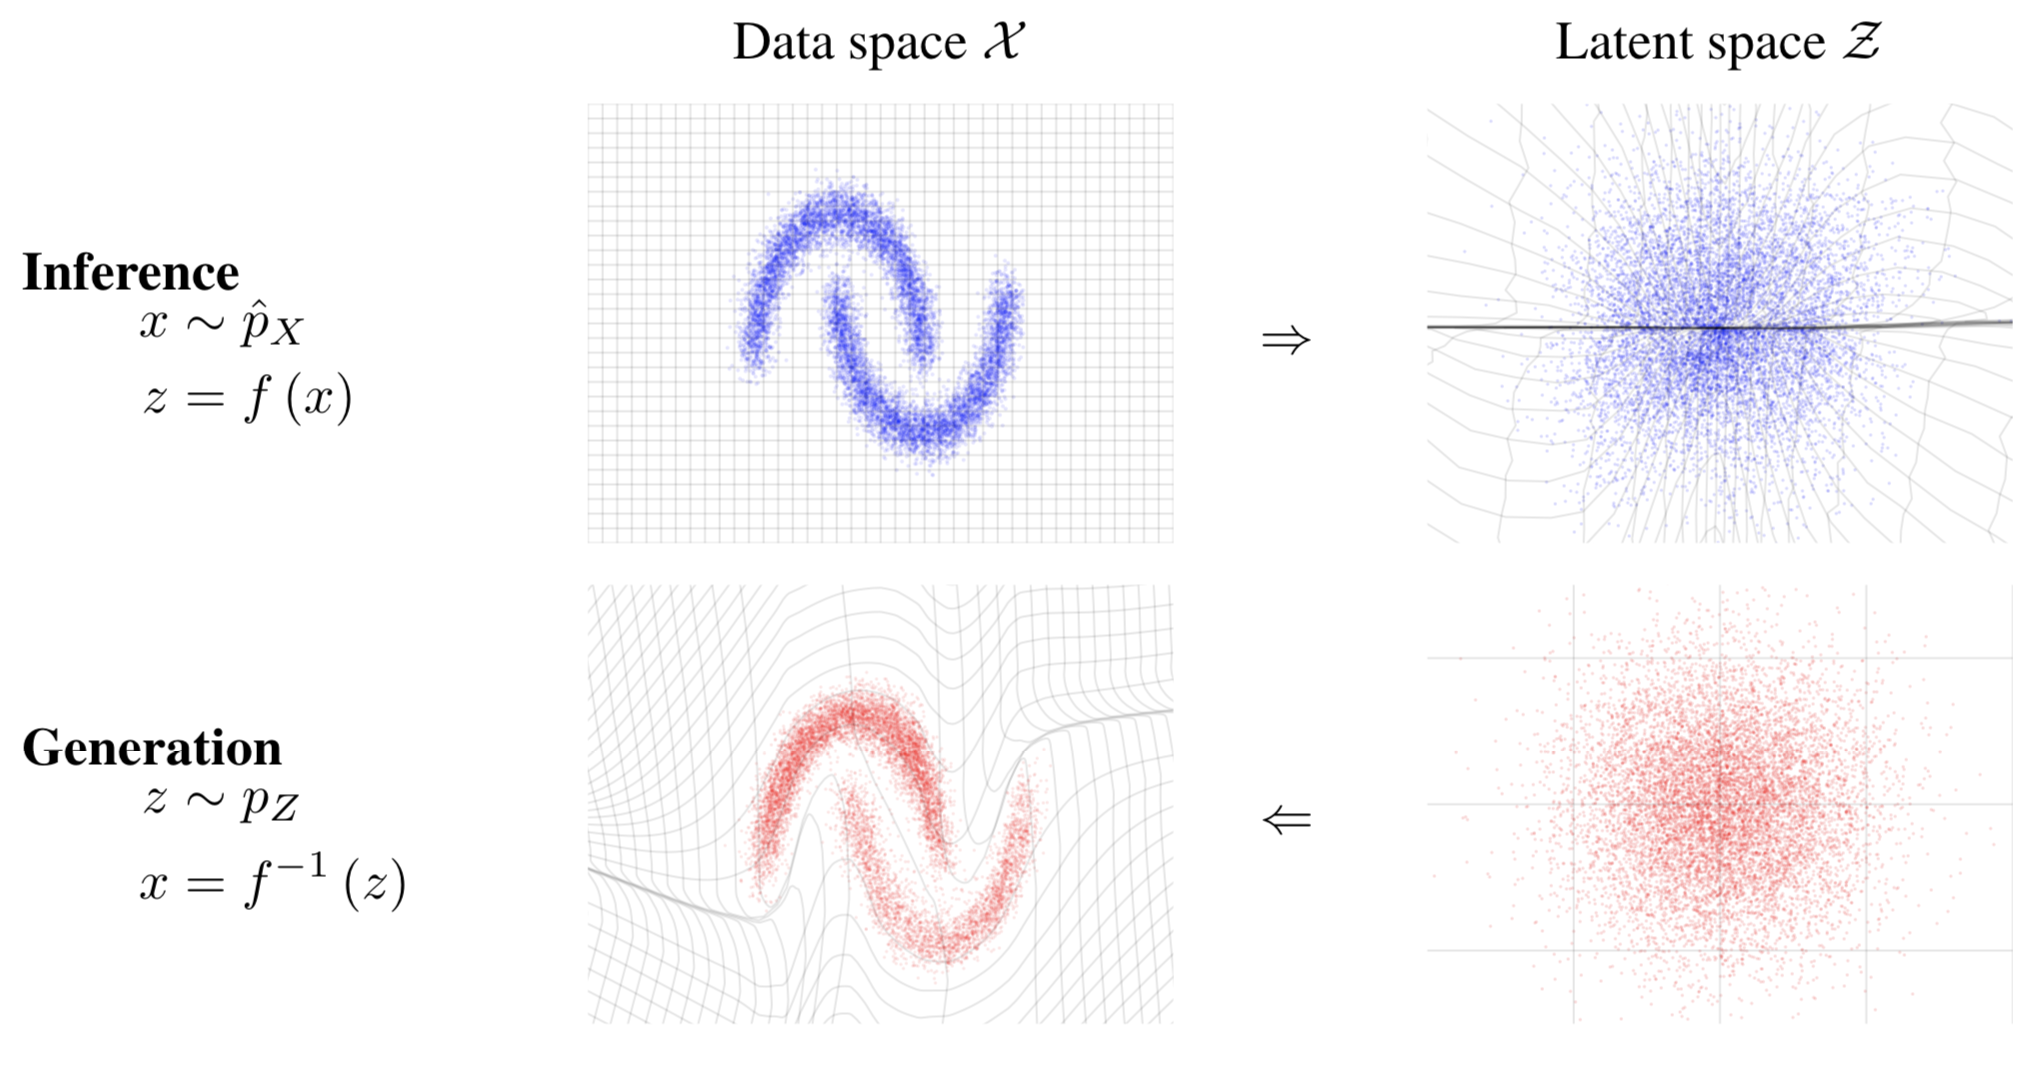
\includegraphics[width=0.85\linewidth]{figs/flows_how2}
	\end{figure}
	\vspace{-0.5cm}
	\begin{block}{Log likelihood}
		\vspace{-0.5cm}
		\[
			\log p(\bx | \btheta) = \log p(\bff_K \circ \dots \circ \bff_1(\bx)) + \sum_{k=1}^K\log |\det (\bJ_{\bff_k})|
		\]
	\end{block}
	\myfootnotewithlink{https://arxiv.org/abs/1605.08803}{Dinh L., Sohl-Dickstein J., Bengio S. Density estimation using Real NVP, 2016} 
\end{frame}
%=======
\begin{frame}{Recap of previous lecture}
	\begin{block}{Forward KL for flow model}
	  	\vspace{-0.1cm}
		\[
			\log p(\bx|\btheta) = \log p(\bff_{\btheta}(\bx)) + \log  |\det (\bJ_\bff)|
		\]
		\vspace{-0.3cm}
	\end{block}
	\begin{block}{Reverse KL for flow model}
  		\vspace{-0.1cm}
		\[
			KL(p || \pi)  = \bbE_{p(\bz)} \left[  \log p(\bz) -  \log |\det (\bJ_\bg)| - \log \pi(\bg_{\btheta}(\bz)) \right]
		\]
		\vspace{-0.5cm}
	\end{block}
	\begin{block}{Flow KL duality}
	  	\vspace{-0.3cm}
		\[
			\argmin_{\btheta} KL(\pi(\bx) || p(\bx | \btheta)) = \argmin_{\btheta} KL(p(\bz | \btheta) || p(\bz))
		\]
		\vspace{-0.3cm}
		\begin{itemize}
			\item $p(\bz)$ is a base distribution; $\pi(\bx)$ is a data distribution;
			\item $\bz \sim p(\bz)$, $\bx = \bg_{\btheta}(\bz)$, $\bx \sim p(\bx| \btheta)$;
			\item $\bx \sim \pi(\bx)$, $\bz = \bff_{\btheta}(\bx)$, $\bz \sim p(\bz | \btheta)$.
		\end{itemize}
	\end{block}
	\myfootnotewithlink{https://arxiv.org/abs/1912.02762}{Papamakarios G. et al. Normalizing flows for probabilistic modeling and inference, 2019} 
\end{frame}
%=======
\begin{frame}{Recap of previous lecture}
	\vspace{-0.5cm}
	\begin{block}{Flow log-likelihood}
		\vspace{-0.3cm}
		\[
			\log p(\bx|\btheta) = \log p(\bff_{\btheta}(\bx)) + \log  |\det (\bJ_\bff)|
		\]
		\vspace{-0.5cm}
	\end{block}
	The main challenge is a determinant of the Jacobian.
	\begin{block}{Linear flows}	
		\vspace{-0.2cm}
		\[
			\bz = \bff_{\btheta}(\bx) = \bW \bx, \quad \bW \in \bbR^{m \times m}, \quad \btheta = \bW, \quad \bJ_\bff = \bW^T
		\]
	\end{block}
	\vspace{-0.3cm}
	\begin{itemize}
		\item LU-decomposition
		\[
			\bW = \mathbf{P} \bL \bU.
		\]
		\item QR-decomposition
		\[
			\bW = \bQ \mathbf{R}.
		\]
	\end{itemize}
	Decomposition should be done only once in the beggining. Next, we fit decomposed matrices ($\bP/\bL/\bU$ or $\bQ/\bR$).
	\myfootnote{\href{https://arxiv.org/abs/1807.03039}{Kingma D. P., Dhariwal P. Glow: Generative Flow with Invertible 1x1 Convolutions, 2018}  \\
	\href{https://arxiv.org/abs/1901.11137}{Hoogeboom E., et al. Emerging convolutions for generative normalizing flows, 2019}
	}
\end{frame}
%=======
\begin{frame}{Recap of previous lecture}
	Consider an autoregressive model
	\vspace{-0.3cm}
	{\small
		\[
		p(\bx | \btheta) = \prod_{j=1}^m p(x_j | \bx_{1:j - 1}, \btheta), \quad
		p(x_j | \bx_{1:j - 1}, \btheta) = \mathcal{N} \left(\mu_j(\bx_{1:j-1}), \sigma^2_j (\bx_{1:j-1})\right).
		\]
	}
	\vspace{-0.5cm}
	\begin{block}{Gaussian autoregressive NF}
		\vspace{-0.5cm}
		\begin{align*}
			\bx &= \bg_{\btheta}(\bz) \quad \Rightarrow \quad {\color{violet} x_j} = \sigma_j ({\color{violet} \bx_{1:j-1}}) \cdot {\color{teal} z_j} + \mu_j({\color{violet} \bx_{1:j-1}}). \\
			\bz &= \bff_{\btheta}(\bx) \quad \Rightarrow \quad {\color{teal} z_j} = \left({\color{violet}x_j} - \mu_j({\color{violet}\bx_{1:j-1}}) \right) \cdot \frac{1}{ \sigma_j ({\color{violet}\bx_{1:j-1}})}.
		\end{align*}
		\vspace{-0.5cm}
	\end{block}
	\begin{itemize}
		\item We have an \textbf{invertible} and \textbf{differentiable} transformation from $p(\bz)$ to $p(\bx | \btheta)$.
		\item Jacobian of such transformation is triangular!
	\end{itemize}
	Generation function $\bg_{\btheta}(\bz)$ is \textbf{sequential}. \\ Inference function $\bff_{\btheta}(\bx)$ is \textbf{not sequential}.
	
	\myfootnotewithlink{https://arxiv.org/abs/1705.07057}{Papamakarios G., Pavlakou T., Murray I. Masked Autoregressive Flow for Density Estimation, 2017} 
\end{frame}
%=======
\begin{frame}{Outline}
    \tableofcontents
\end{frame}
%=======
\section{RealNVP: coupling layer}
%=======
\begin{frame}{RealNVP}
	\vspace{-0.5cm}
	Let split $\bx$ and $\bz$ in two parts: 
	\[
		\bx = [\bx_1, \bx_2] = [\bx_{1:d}, \bx_{d+1:m}]; \quad \bz = [\bz_1, \bz_2] = [\bz_{1:d}, \bz_{d+1:m}].
	\]
	\vspace{-0.7cm}
	\begin{block}{Coupling layer}
		\vspace{-0.7cm}
		\[
			\begin{cases} \bx_1 = \bz_1; \\ \bx_2 = \bz_2 \odot \bsigma_{\btheta}(\bz_1) + \bmu_{\btheta}(\bz_1).\end{cases}  
			\begin{cases} \bz_1 = \bx_1; \\ \bz_2 = \left(\bx_2 - \bmu_{\btheta}({\color{olive}\bx_1}) \right) \odot \frac{1}{\bsigma_{\btheta}({\color{olive}\bx_1})}.\end{cases}
		\]
	\end{block}
	\vspace{-0.5cm}
	\begin{block}{Image partitioning}
		
		\begin{minipage}[t]{0.5\columnwidth}
			\begin{figure}
				\centering
				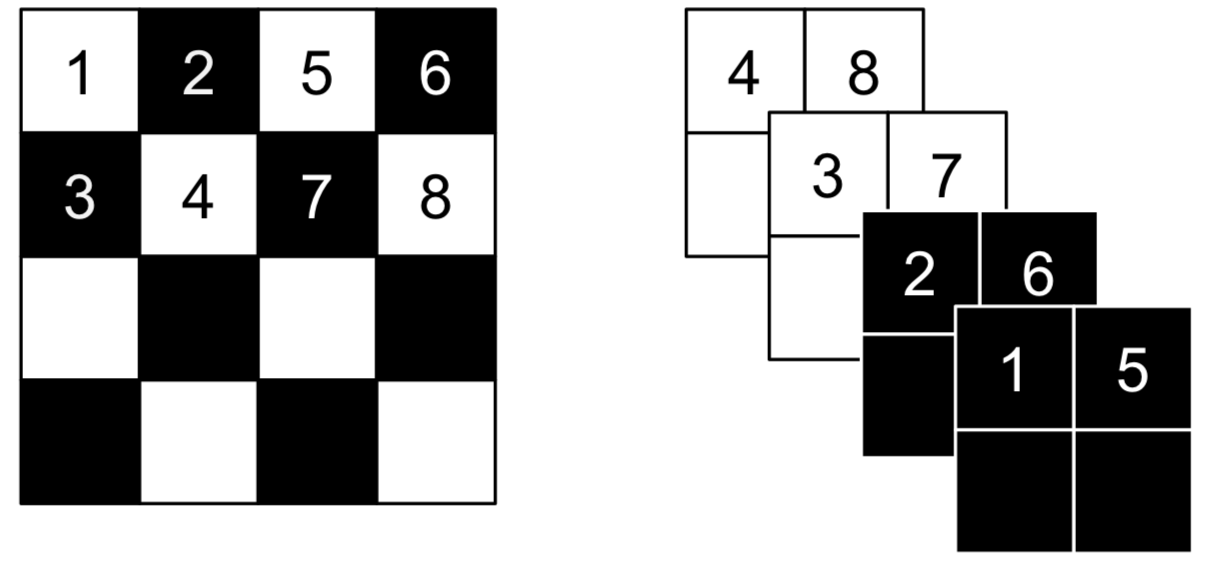
\includegraphics[width=\linewidth]{figs/realnvp_masking.png}
			\end{figure}
		\end{minipage}% 
		\begin{minipage}[t]{0.5\columnwidth}
			\begin{itemize}
				\item Checkerboard ordering uses masking.
				\item Channelwise ordering uses splitting.
			\end{itemize}
		\end{minipage}
	\end{block}
	\vspace{-0.5cm}
	\myfootnotewithlink{https://arxiv.org/abs/1605.08803}{Dinh L., Sohl-Dickstein J., Bengio S. Density estimation using Real NVP, 2016} 
\end{frame}
%=======
\begin{frame}{RealNVP}
	\begin{block}{Coupling layer}
		\vspace{-0.7cm}
		\[
		 \begin{cases} {\color{violet}\bx_1} = {\color{teal}\bz_1}; \\ {\color{violet}\bx_2} = {\color{teal}\bz_2} \odot \bsigma_{\btheta}({\color{teal}\bz_1}) + \bmu_{\btheta}({\color{teal}\bz_1}).\end{cases}  
		\begin{cases} {\color{teal}\bz_1} ={\color{violet} \bx_1}; \\ {\color{teal}\bz_2} = \left({\color{violet}\bx_2} - \bmu_{\btheta}({\color{violet}\bx_1}) \right) \odot \frac{1}{\bsigma_{\btheta}({\color{violet}\bx_1})}.\end{cases}
		\]
		Estimating the density takes 1 pass, sampling takes 1 pass!
	\end{block}
	\begin{block}{Jacobian}
		\vspace{-0.5cm}
		\[
		\det \left( \frac{\partial \bz}{\partial \bx} \right) = \det 
		\begin{pmatrix}
			\bI_d & 0_{d \times m - d} \\
			\frac{\partial \bz_2}{\partial \bx_1} & \frac{\partial \bz_2}{\partial \bx_2}
		\end{pmatrix} = \prod_{j=1}^{m - d} \frac{1}{\sigma_j(\bx_1)}.
		\]
		\vspace{-0.5cm}
	\end{block}
	\begin{block}{Gaussian AR NF}
		\vspace{-0.6cm}
		\begin{align*}
			\bx &= \bg_{\btheta}(\bz) \quad \Rightarrow \quad {\color{violet}x_j} = \sigma_j ({\color{violet}\bx_{1:j-1}}) \cdot {\color{teal} z_j} + \mu_j({\color{violet}\bx_{1:j-1}}). \\
			\bz &= \bff_{\btheta}(\bx) \quad \Rightarrow \quad {\color{teal} z_j} = \left({\color{violet} x_j} - \mu_j({\color{violet}\bx_{1:j-1}}) \right) \cdot \frac{1}{\sigma_j ({\color{violet} \bx_{1:j-1}}) }.
		\end{align*}
		\vspace{-0.5cm}
	\end{block}
	How to get RealNVP coupling layer from gaussian AR NF?
	
	\myfootnotewithlink{https://arxiv.org/abs/1605.08803}{Dinh L., Sohl-Dickstein J., Bengio S. Density estimation using Real NVP, 2016} 
\end{frame}
%=======
\begin{frame}{Glow samples}
	Glow model: coupling layer + linear flows (1x1 convs)
	\begin{figure}
		\centering
		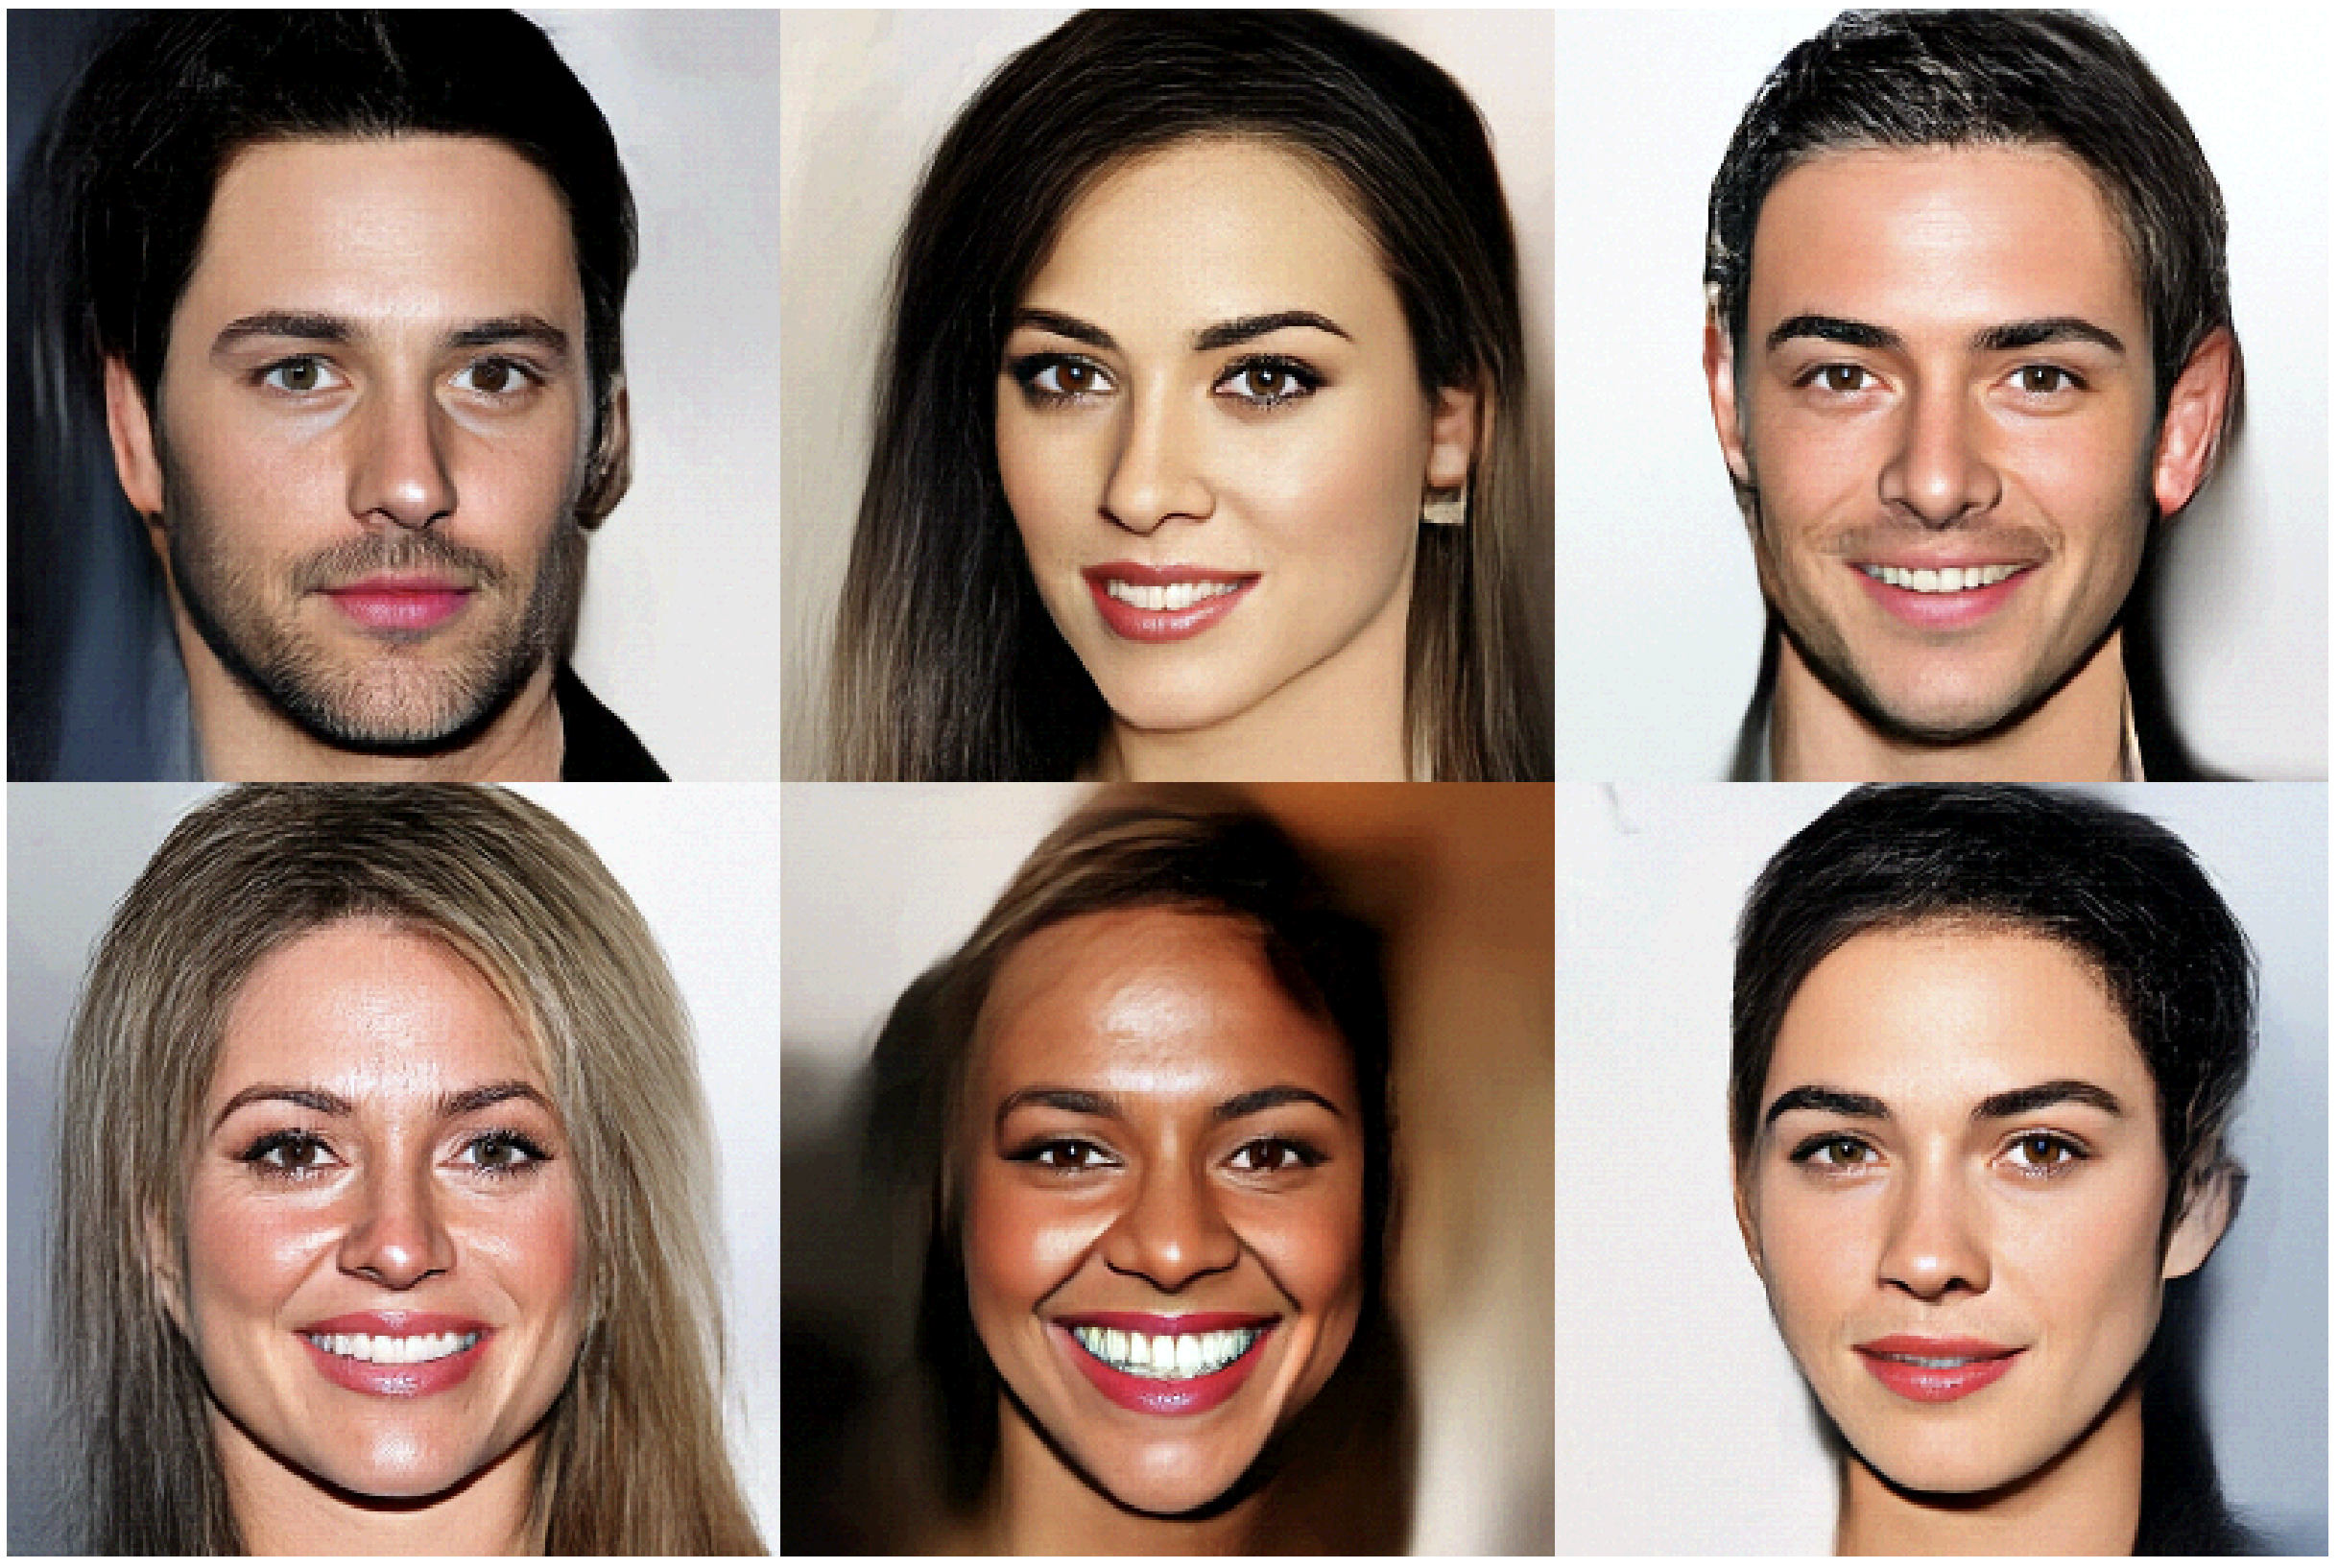
\includegraphics[width=0.9\linewidth]{figs/glow_faces.png}
	\end{figure}
	\myfootnotewithlink{https://arxiv.org/abs/1807.03039}{Kingma D. P., Dhariwal P. Glow: Generative Flow with Invertible 1x1 Convolutions, 2018}
\end{frame}
%=======
\begin{frame}{Venn diagram for Normalizing flows}
	
	\begin{figure}
		\centering
		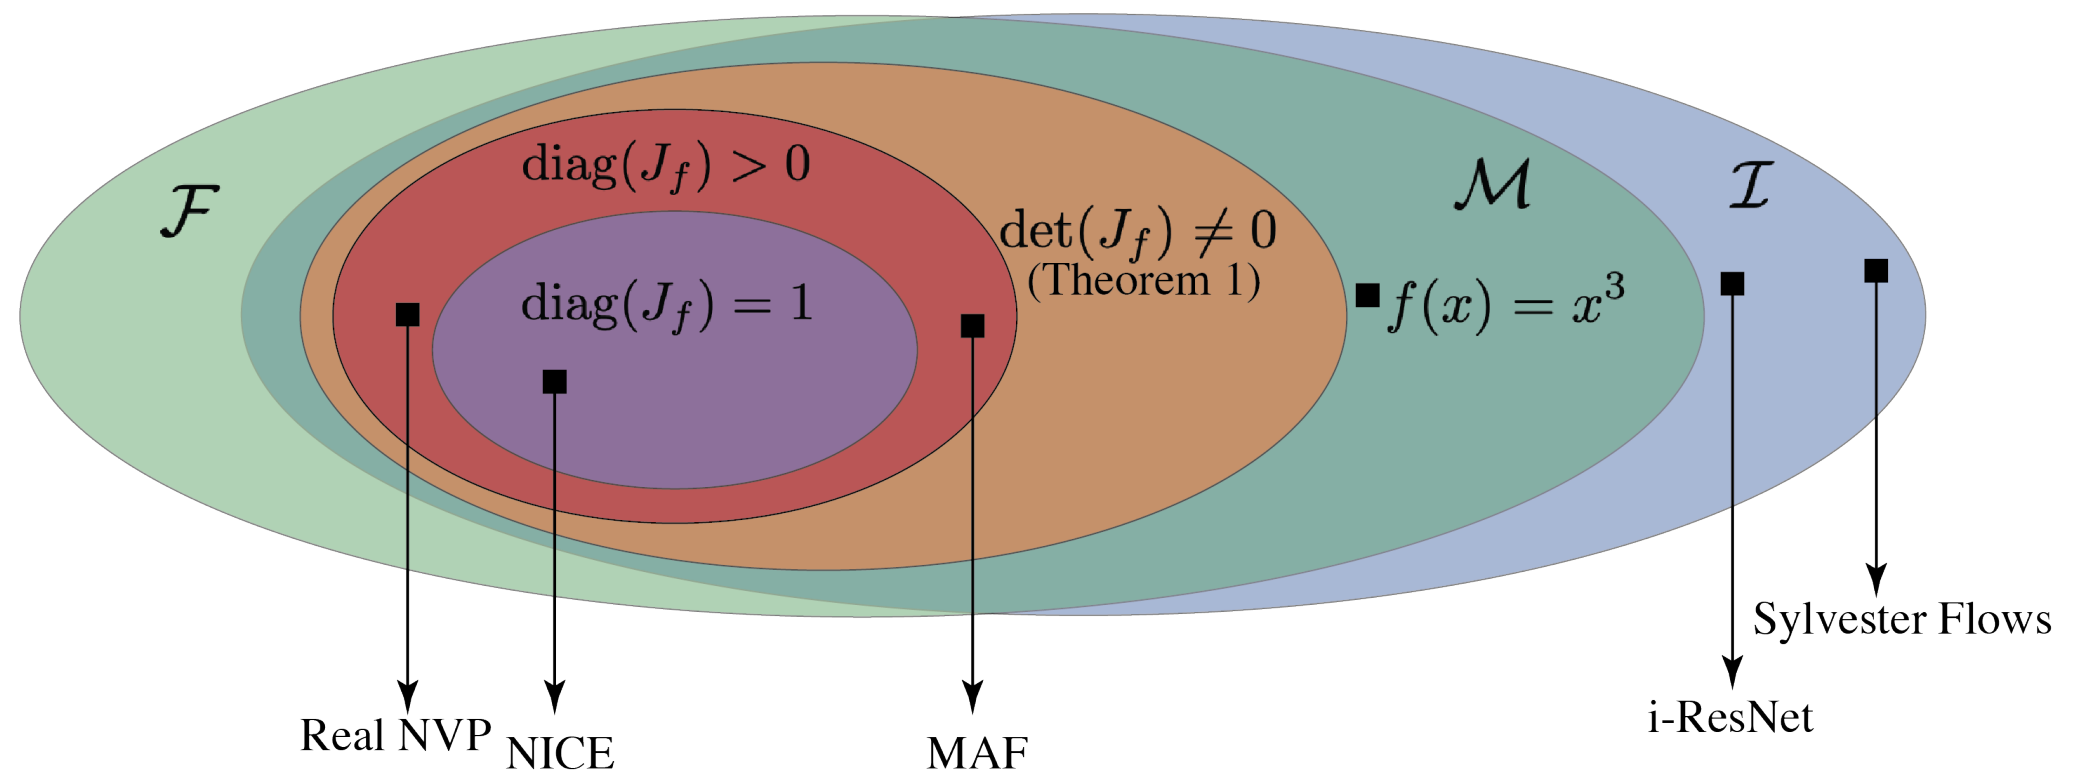
\includegraphics[width=\linewidth]{figs/venn_diagram}
	\end{figure}
	\begin{itemize}
		\item $\cI$ -- invertible functions.
		\item $\cF$ -- continuously differentiable functions whose Jacobian is lower triangular.
		\item $\cM$ -- invertible functions from $\cF$.
	\end{itemize}
	\myfootnotewithlink{https://arxiv.org/abs/1907.07945}{Song Y., Meng C., Ermon S. Mintnet: Building invertible neural networks with masked convolutions, 2019}
\end{frame}
%=======
\section{Continuous-in-time normalizing flows}
%=======
\begin{frame}{Continuous-in-time normalizing flows}
	\vspace{-0.3cm}
	\begin{block}{Discrete-in-time NF}
		Previously we assume that the time axis is discrete:
		\vspace{-0.3cm}
		  \[
			  \bz_{t+1} = \bff_{\btheta}(\bz_t); \quad \log p(\bz_{t+1}) = \log p(\bz_{t}) - \log \left| \det \frac{\partial \bff_{\btheta}(\bz_t)}{\partial \bz_{t}} \right| .
		  \]
		\vspace{-0.6cm}
	\end{block}
	Let assume the more general case of continuous time. It means that we will have the dynamic function $\bz(t)$.
	\begin{block}{Continuous-in-time dynamics}
		Consider Ordinary Differential Equation (ODE)
		\vspace{-0.3cm}
		\begin{align*}
		   \frac{d \bz(t)}{dt} &= \bff_{\btheta}(\bz(t), t); \quad \text{with initial condition }\bz(t_0) = \bz_0. \\
		   \bz(t_1) &= \int^{t_1}_{t_0} \bff_{\btheta}(\bz(t), t) d t  + \bz_0 \approx \text{ODESolve}(\bz(t_0), \bff_{\btheta}, t_0,t_1).
		\end{align*}
		\vspace{-0.6cm}
	\end{block}
	Here we need to define the computational procedure $\text{ODESolve}(\bz(t_0), \bff_{\btheta}, t_0,t_1)$.
	\myfootnotewithlink{https://arxiv.org/abs/1810.01367}{Grathwohl W. et al. FFJORD: Free-form Continuous Dynamics for Scalable Reversible Generative Models, 2018}  
\end{frame}
%=======
\begin{frame}{Continuous-in-time normalizing flows}
	\begin{block}{Euler update step}
		\vspace{-0.5cm}
		\[
		    \frac{\bz(t + \Delta t) - \bz(t)}{\Delta t} = \bff_{\btheta}(\bz(t), t) \,\, \Rightarrow \,\, \bz(t + \Delta t) = \bz(t) + \Delta t \cdot \bff_{\btheta}(\bz(t), t)
		\]
		\vspace{-0.5cm}
	\end{block}
	\textbf{Note:} Euler method is the simplest version of ODESolve that is unstable in practice.  It is possible to use more sophisticated methods (e.x. Runge-Kutta methods).
	\begin{minipage}[t]{0.4\columnwidth}
		\begin{figure}
			\centering
			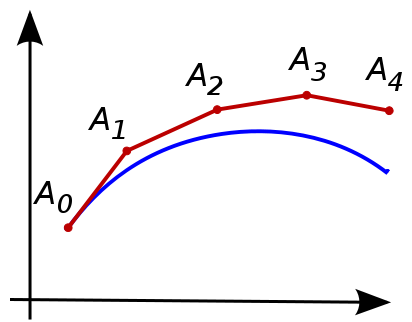
\includegraphics[width=0.7\linewidth]{figs/euler}
		\end{figure}
	\end{minipage}%
	\begin{minipage}[t]{0.6\columnwidth}
		\vspace{-0.2cm}
		\begin{figure}
			\centering
			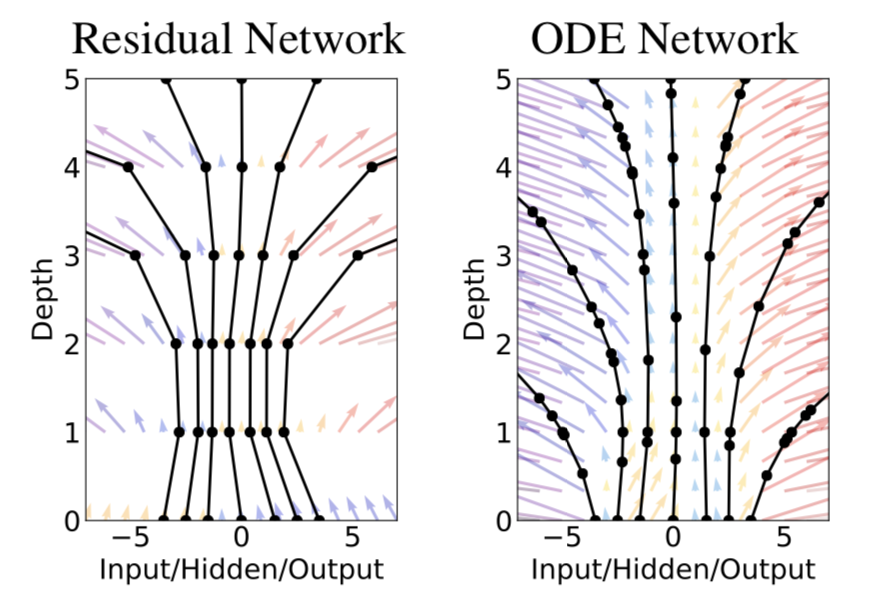
\includegraphics[width=0.9\linewidth]{figs/resnet_vs_neural_ode.png}
		\end{figure}
	\end{minipage}
	
	\myfootnotewithlink{https://arxiv.org/abs/1806.07366}{Chen R. T. Q. et al. Neural Ordinary Differential Equations, 2018}   

\end{frame}
%=======
\begin{frame}{Continuous-in-time Normalizing Flows}
	\vspace{-0.5cm}
	\begin{block}{Neural ODE}
		\vspace{-0.5cm}
		\begin{align*}
  \frac{d \bz(t)}{dt} &= \bff_{\btheta}(\bz(t), t); \quad \text{with initial condition }\bz(t_0) = \bz_0
		\end{align*}
		\vspace{-0.8cm}
	\end{block}
	\begin{minipage}[t]{0.6\columnwidth}
		\begin{itemize}
			\item Let $\bz(t_0)$ will be a random variable with some density function $p(\bz(t_0))$.
		 	\item Then $\bz(t_1)$ will be also a random variable with some other density function $p(\bz(t_1))$.
			\item We could say that we have the joint density function $p(\bz(t), t)$.
			\item What is the difference between $p(\bz(t), t)$ and $p(\bz, t)$?
		\end{itemize}
	\end{minipage}%
	\begin{minipage}[t]{0.4\columnwidth}	
		\begin{figure}
			\centering
			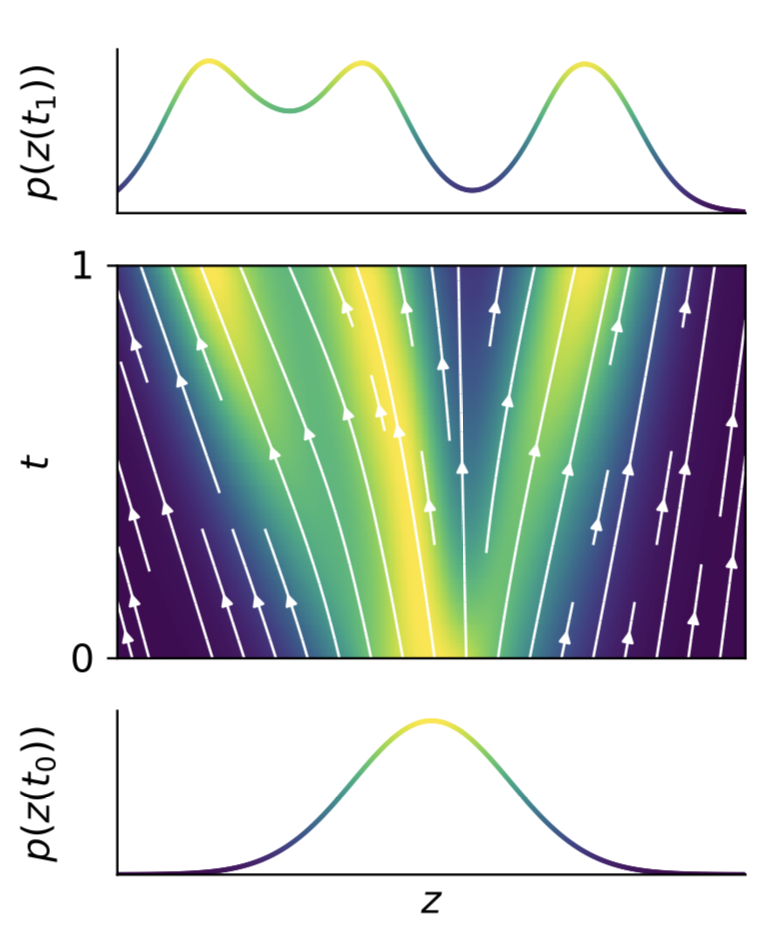
\includegraphics[width=\linewidth]{figs/cnf_flow.png}
		\end{figure}
	\end{minipage}
	\myfootnotewithlink{https://arxiv.org/abs/1810.01367}{Grathwohl W. et al. FFJORD: Free-form Continuous Dynamics for Scalable Reversible Generative Models, 2018}  
\end{frame}
%=======
\begin{frame}{Continuous-in-time Normalizing Flows}
	Let say that $p(\bz, t_0)$ is the base distribution (e.x. standard Normal) and $p(\bz, t_1)$ is the desired model distribution $p(\bx | \btheta)$.
	\begin{block}{Theorem (Picard)}
		If $\bff$ is uniformly Lipschitz continuous in $\bz$ and continuous in $t$, then the ODE has a \textbf{unique} solution.
	\end{block}
	It means that we are able \textbf{uniquely revert} our ODE. 
	\begin{block}{Forward and inverse transforms}
		\vspace{-0.7cm}
		\begin{align*}
			\bx &= \bz(t_1) = \bz(t_0) + \int_{t_0}^{t_1} \bff_{\btheta}(\bz(t), t) dt \\
			\bz &= \bz(t_0) = \bz(t_1) + \int_{t_1}^{t_0} \bff_{\btheta}(\bz(t), t) dt
		\end{align*}
		\vspace{-0.7cm}
	\end{block}
	\textbf{Note:} Unlike discrete-in-time NF, $\bff$ does not need to be bijective (uniqueness guarantees bijectivity).
	\myfootnotewithlink{https://arxiv.org/abs/1806.07366}{Chen R. T. Q. et al. Neural Ordinary Differential Equations, 2018}   
\end{frame}
%=======
\begin{frame}{Continuous-in-time Normalizing Flows}
	\begin{block}{What do we need?}
		\begin{itemize}
			\item We need the way to compute $p(\bz, t)$ at any moment $t$.
			\item We need the way to find the optimal parameters $\btheta$ of the dynamic $\bff_{\btheta}$.
		\end{itemize}
	\end{block}
	\vspace{-0.3cm}
	\begin{block}{Theorem (Kolmogorov-Fokker-Planck: special case)}
		If $\bff$ is uniformly Lipschitz continuous in $\bz$ and continuous in $t$, then
		\[
			\frac{d \log p(\bz(t), t)}{d t} = - \text{tr} \left( \frac{\partial \bff_{\btheta}(\bz(t), t)}{\partial \bz(t)} \right).
		\]
		\[
			\log p(\bz(t_1), t_1) = \log p(\bz(t_0), t_0) - \int_{t_0}^{t_1} \text{tr}  \left( \frac{\partial \bff_{\btheta}(\bz(t), t)}{\partial \bz(t)} \right) dt.
		\]
	\end{block}
	It means that if we have the value $\bz_0 = \bz(t_0)$ then the solution of the ODE will give us the density at the moment $t_1$.
	\myfootnotewithlink{https://arxiv.org/abs/1806.07366}{Chen R. T. Q. et al. Neural Ordinary Differential Equations, 2018}   
\end{frame}
%=======
\begin{frame}{Continuous-in-time Normalizing Flows}
	\begin{block}{Forward transform + log-density}
		\vspace{-0.7cm}
		\begin{align*}
				\bx &= \bz + \int_{t_0}^{t_1} \bff_{\btheta}(\bz(t), t) dt \\
				\log p(\bx | \btheta) &= \log p(\bz) - \int_{t_0}^{t_1} \text{tr} \left( \frac{\partial \bff_{\btheta}(\bz(t), t)}{\partial \bz(t)} \right) dt
		\end{align*}
		Here $p(\bx | \btheta) = p(\bz(t_1), t_1)$, $p(\bz) = p(\bz(t_0), t_0)$.
	\end{block}
	\begin{itemize}
		\item \textbf{Discrete-in-time NF}: evaluation of determinant of the Jacobian costs $O(m^3)$ (we need invertible $\bff$).
		\item \textbf{Continuous-in-time NF}: getting the trace of the Jacobian costs $O(m^2)$ (we need smooth $\bff$).
	\end{itemize}
	\begin{block}{Why $O(m^2)$?}
		$\text{tr} \left( \frac{\partial \bff_{\btheta}(\bz(t))}{\partial \bz(t)} \right)$ costs $O(m^2)$ ($m$ evaluations of $\bff$), since we have to compute a derivative for each diagonal element. It is possible to reduce cost from $O(m^2)$ to $O(m)$!
	\end{block}
	\myfootnotewithlink{https://arxiv.org/abs/1806.07366}{Chen R. T. Q. et al. Neural Ordinary Differential Equations, 2018}   
\end{frame}
%=======
\begin{frame}{Continuous-in-time Normalizing Flows}
	\begin{block}{Hutchinson's trace estimator}
		If $\bepsilon \in \bbR^m$ is a random variable with $\mathbb{E} [\bepsilon] = 0$ and $\text{cov} (\bepsilon) = \bI$, then
		\vspace{-0.3cm}
		\begin{multline*}
		    \text{tr}(\mathbf{A}) = \text{tr}\left(\mathbf{A} \cdot {\color{olive}\bI} \right) = \text{tr}\left(\mathbf{A} \cdot {\color{olive}\mathbb{E}_{p(\bepsilon)} \left[ \bepsilon \bepsilon^T \right]} \right) = \\ 
		    =  \mathbb{E}_{p(\bepsilon)} \left[  \text{tr}\left(  \mathbf{A}  \bepsilon \bepsilon^T \right) \right] =  \mathbb{E}_{p(\bepsilon)} \left[ {\color{violet} \bepsilon^T \mathbf{A}} \bepsilon  \right]
		\end{multline*}
		\vspace{-0.6 cm}
	\end{block}
	Jacobian vector products ${\color{violet}\bv^T \frac{\partial f}{\partial \bz}}$ can be computed for approximately the same cost as evaluating $\bff$ (\texttt{torch.autograd.functional.jvp}).
	\begin{block}{FFJORD density estimation}
		\vspace{-0.8cm}
		\begin{multline*}
		    \log p(\bz(t_1)) = \log p(\bz(t_0)) - \int_{t_0}^{t_1} \text{tr}  \left( \frac{\partial \bff_{\btheta}(\bz(t), t)}{\partial \bz(t)} \right) dt = \\ = \log p(\bz(t_0)) - \mathbb{E}_{p(\bepsilon)} \int_{t_0}^{t_1} \left[ {\color{violet}\bepsilon^T \frac{\partial \bff}{\partial \bz}} \bepsilon \right] dt.
		\end{multline*}
	\end{block}
	\myfootnotewithlink{https://arxiv.org/abs/1810.01367}{Grathwohl W. et al. FFJORD: Free-form Continuous Dynamics for Scalable Reversible Generative Models, 2018} 
\end{frame}
%=======
\begin{frame}{Summary}
	\begin{itemize}
		\item The RealNVP coupling layer is an effective type of NF (special case of AR NF) that has fast inference and generation modes.
		\vfill
		\item Continuous-in-time NF uses neural ODE to define continuous dynamic $\bz(t)$. It has less functional restrictions.
		\vfill 
		\item Kolmogorov-Fokker-Planck theorem allows to calculate $\log p(\bz, t)$ at arbitrary moment $t$.
		\vfill
		\item FFJORD model makes such kind of NF scalable.
	\end{itemize}
\end{frame}
\end{document} 